\chapter{A Full-System Co-Simulator for Storage Subsystem Evaluation}
%TODO: A Full-System Co-Simulation Environment for Storage Subsystem Evaluation
\label{ch:5}

In this chapter, an OS-based full-system co-simulation environment based on the proposed virtual storage device and real computer system co-simulation methodology is described. The proposed full-system co-simulator can be used for performing storage subsystem evaluations in full-system contexts. Specifically, the virtual storage device can be simulated together with the entire OS and benchmark applications so that it can be evaluated using realistic real-world workloads and system-level measurement metrics.

The OS chosen for the implementation of the proposed full-system co-simulator is the Ubuntu Linux version 11.0 with kernel version 3.0.0-19~\cite{Ubuntu:2013}. The CPU architecture is the Intel x86 architecture. The concepts and modifications described in this chapter should also be applicable to other OS's and CPU architectures. Figure~\ref{fig:ch5-full-system-simulator} illustrates the overall architecture of the proposed full-system co-simulator. There are two key parts to the design of the proposed full-system co-simulator. The first part is related to the modifications made to the task scheduling and timekeeping infrastructures of the Linux kernel for controlling the state of the OS. These modifications are related to the ability for co-simulating the virtual storage device and physical computer system in the discrete-time domain. The related modules are shown in the gray blocks in Figure~\ref{fig:ch5-full-system-simulator} and are discussed in section~\ref{sec:managing-linux-OS-state} and \ref{sec:controlling-current-system-time}. The second part is related to the emulating of the virtual storage device to the OS. The related modules are shown in the white blocks with solid lines and are discussed in section~\ref{sec:storage-device-simulation-module} and \ref{sec:direct-backing-storage}.

\begin{figure}[htpb]
	\centering
	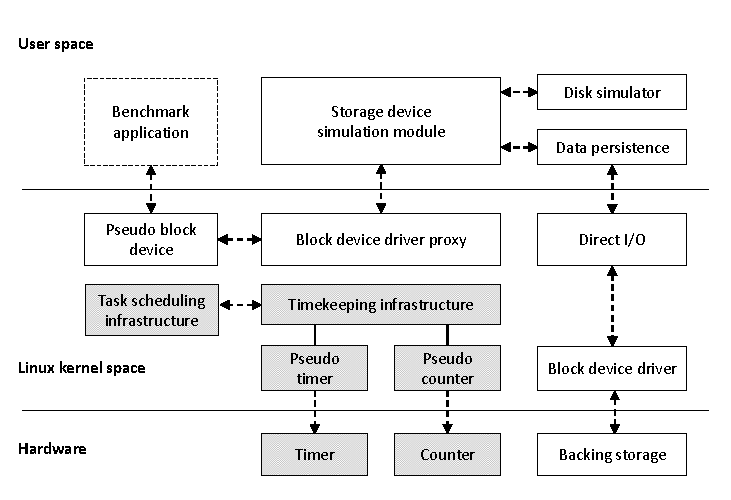
\includegraphics[width=1\textwidth]{figures/ch5-full-system-simulator.pdf}
	\caption{\label{fig:ch5-full-system-simulator}Overview of the proposed full-system co-simulator.}
\end{figure}

\section{Controlling the State of the Linux Operating System}
\label{sec:managing-linux-OS-state}

The state of the Linux OS can be viewed as the combined state of the user space processes, the kernel space threads, and the current system time. Here, the user space processes and the kernel space threads are collectively called the normal OS processes. In comparison, the processes responsible for simulating the storage device are called the simulator processes. The state of the Linux OS can be paused by blocking all normal OS processes from executing on the CPU and stopping the advancement of the hardware timer and counters.

The task scheduler of the Linux kernel is modified so that the normal OS processes can be distinguished from the simulator processes. Whenever the simulator processes are executing, the Linux OS will be put into the paused state. Because of the pausing made to the OS state, the behaviors of the normal processes, and therefore the system-level behaviors that are of interest, will not be affected by the simulator processes.

\begin{figure}[htpb]
	\centering
	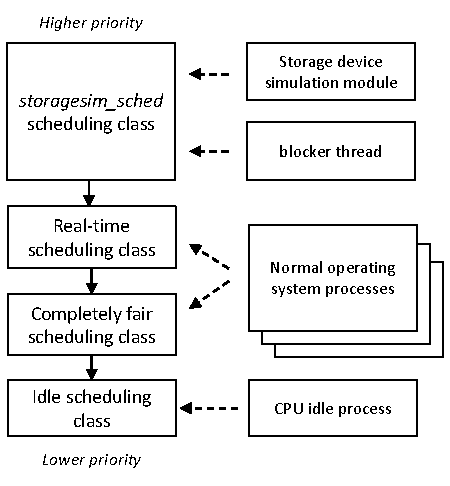
\includegraphics[width=0.6\textwidth]{figures/ch5-scheduling-classes.pdf}
	\caption{\label{fig:ch5-scheduling-classes}Scheduling classes in the Linux task scheduling infrastructure.}
\end{figure}

As illustrated in Figure~\ref{fig:ch5-scheduling-classes}, the task scheduler of the Linux OS is made up of several scheduling classes (\textit{struct sched_class}, defined in \textit{include/linux/sched.h}). In the stock Linux kernel, the normal OS processes can belong to either the real-time (RT) scheduling class (\textit{rt_sched_class}, implemented in \textit{kernel/sched_fair.c}) or the completely fair scheduling (CFS) class (\textit{fair_sched_class}, implemented in \textit{kernel/sched_fair.c})~\cite{Bovet:2005}, \cite{Love:2010}. The RT scheduling class has higher priority than the CFS class. That is, processes in the RT scheduling class always get to run before the processes in the CFS class.

In the proposed full-system co-simulator, a special \textit{storagesim_sched} scheduling class is implemented and given the highest priority in the task scheduler. The simulator processes, such as the processes that are responsible for simulating the storage device, are registered under the \textit{storagesim_sched} scheduling class. Therefore, whenever the storage device simulation module has to handle the simulation of the virtual storage device, it will be scheduled immediately and blocks all normal processes from running. Furthermore, when the task scheduler selects a process from the \textit{storagesim_sched} scheduling class, the task scheduler will know that the process is one of the simulator processes and will make a request to the modified timekeeping infrastructure to pause the current system time. The preventing of the normal OS processes from running and the pausing of the current system time effectively puts the Linux OS into the paused mode. To bring the OS base to the normal running state when the normal OS processes are selected again for running, the current system time will be set to progress normally according to the wall-clock time.

Because the normal OS processes are scheduled according to the same scheduling algorithms in the unmodified Linux kernel (i.e., by the RT and the CFS scheduling classes), the multi-tasking behavior of the Linux OS is preserved in the proposed full-system co-simulator.

When the simulator process releases itself form using the CPU, it is possible that it still requires that the OS is kept in the paused mode for some indefinite amount of time. For example, when the storage device simulation module needs to read some data from the backing storage to prepare for an I/O response, it will be put into the I/O wait state when waiting for the response from the backing storage. During this wait period on the backing storage, the state of the Linux OS should still remain in the paused mode even if there is no simulator process needs to use the CPU. That is, the Linux OS cannot be put back to the running mode yet. Otherwise, when the storage device simulation module finally receives the actual data from the backing storage and is ready to reply the I/O response to the OS, the OS state might have already have advanced past the intended system time at which the I/O response should be replied at.

To handle the need for keeping the OS in the paused mode while waiting for the data from the backing storage, a kernel space ``blocker thread'' is introduced. The blocker thread is a kernel thread that runs an infinite idle loop and is registered as the lowest priority thread in the \textit{storagesim_sched} scheduling class. The blocker thread can be enabled or disabled by the simulator processes through a system call. The storage device simulation module will enable the blocker thread before issuing requests to the backing storage and disables it after the responses are received.

\section{Controlling the Current System Time}
\label{sec:controlling-current-system-time}

The timekeeping infrastructure of the Linux kernel is responsible for providing two services to the system: (1) Provisioning of the current system time, and (2) Provisioning of a timer service which can be used to schedule callback events in future time points.

Historically, the Linux kernel tracks system time and schedules timer callback events using a periodic timer tick. The internal kernel value \textit{jiffies} records the number of timer ticks since the system is powered on and is incremented at each timer interrupt. Depending on the kernel configuration, the frequency of the timer interrupt is typically between 100Hz to 1000Hz. That is, the resolution of \textit{jiffies} is typically between 1\si{\milli\second} and 10\si{\milli\second}. Due to the coarse resolution of \textit{jiffies}, the proposed full-system co-simulator cannot rely on it to represent the Linux OS state for discrete event simulation. For example, if the Linux OS is put into the running mode at time \textit{t} and runs for 0.5\si{\milli\second} before it makes an I/O request to the virtual storage device, then when switching to the paused mode, the state of the Linux OS should be recorded to be at time \textit{t}+0.5\si{\milli\second}. However, if \textit{jiffies} with resolution of 1\si{\milli\second} is used for representing the current system time of the Linux OS state, it is not possible to represent the OS state at exactly \textit{t}+0.5\si{\milli\second}. Only representing the discrete state of the Linux OS at the \textit{jiffies} granularity (i.e., down to 1\si{\milli\second}) is insufficient for the purpose of storage subsystem evaluation.

A na\"{\i}ve solution would be to increase the resolution of the \textit{jiffies} to a higher resolution. However, the problem with this approach is that it will significantly change the original behavior of the Linux OS. For example, having the \textit{jiffies} at the 1\si{\micro\second} resolution would mean that the hardware timer will need to be interrupting the Linux OS at one million times per second. This will cause the interrupts to consume a lot of additional CPU cycles. Furthermore, even at 1\si{\micro\second} resolution, it could still be too coarse for representing the state of the Linux OS.

\begin{figure}[htpb]
	\centering
	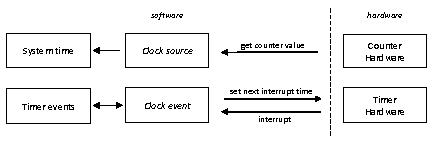
\includegraphics[width=0.95\textwidth]{figures/ch5-clocksource-clockevent.pdf}
	\caption[The \textit{clock source} and \textit{clock event} devices.]{\label{fig:ch5-clocksource-clockevent}The \textit{clock source} and \textit{clock event} devices in the Linux timekeeping infrastructure.}
\end{figure}

Between kernel version 2.6.19 and 2.6.21, a new timekeeping infrastructure was introduced to the Linux kernel~\cite{Stultz:2005}, \cite{GleixnerNiehaus:2006}, \cite{GleixnerMolnar:2006}, \cite{Gleixner:2007}, \cite{Kerrisk:2012}. As illustrated in Figure~\ref{fig:ch5-clocksource-clockevent}, the new timekeeping infrastructure is composed of \textit{clock source} and \textit{clock event} devices. To be able to control the system time in a finer granularity, the proposed full-system co-simulator requires that the Linux kernel is configured to use this new timekeeping infrastructure.

The \textit{clock source} device, defined in \textit{/kernel/time/clocksource.h}, is used to provide the current system time to the timekeeping infrastructure. It utilizes a monotonically increasing hardware counter in the system for measuring elapsed time. When the current time value is needed, the \textit{clock source} device reads the hardware counter and translates the counter value into current system time. The unit of the current system time is in nanoseconds. Depending on the hardware configuration, there could be many available hardware counters in a system. The timekeeping infrastructure will select the most suitable hardware counter to be used as the \textit{clock source} device. The chosen device It is usually the hardware counter with the highest resolution. On the testing platform of the proposed full-system co-simulator, the hardware counter selected is the Time Stamp Counter (TSC)~\cite{Intel:1997}, \cite{wiki:TSC}.

As illustrated in Figure~\ref{fig:ch5-full-system-simulator}, in the proposed full-system co-simulator, the hardware counter selected by the timekeeping infrastructure will be wrapped by a pseudo software counter. Therefore, by controlling the value of the pseudo counter, the current system time perceived by the Linux OS can be controlled. Furthermore, because the TSC counter selected in the test platform has a resolution of a single CPU clock cycle, the current system time part of the Linux OS state can be precisely captured.

The \textit{clock event} device, defined in \textit{/kernel/time/clockevents.h}, is used for providing timer callback service. The timer events in the Linux kernel are sorted in a red-block tree data structure. The most recent timer event will always be programed to the \textit{clock event} device. When programed, the \textit{clock event} device will set the timer hardware in the system. The timer hardware utilized in the testing platform is the Local Advanced Programmable Interrupt Controller (LAPIC) timer. As illustrated in Figure~\ref{fig:ch5-full-system-simulator}, the selected hardware timer is wrapped by a pseudo software timer. Through the pseudo software timer, the full-system co-simulator can know the next time point that a timer event will happen. This knowledge is used by the time-skipping feature to fast-forward the simulation time when the CPU enters the idle loop. The time-skipping feature is discussed in section~\ref{sec:time-skipping}.

By intercepting and controlling the values that the pseudo counter and the pseudo timer provide to the upper layers of the timekeeping infrastructure, the timekeeping infrastructure is modified to support the following operations:

\begin{itemize}
	\item Normal operation when in running mode --- When the Linux OS is in the running mode, the value of the pseudo counter is incremented at the same rate as the real TSC counter. The pseudo counter only needs to be synchronized with the TSC counter when it is being referenced. To the Linux OS, the system time will be progressing at the real-world clock speed. In addition, when timer event is programmed to the pseudo timer, the pseudo timer will set the corresponding timer value the real LAPIC timer.
	
	\item Switch from running mode to paused mode --- When Linux needs to be switched from running mode to paused mode, two steps are performed for proper mode switch operation: (1) Disables the hardware timer and records the remaining time in the pseudo timer. For example, if the pseudo timer is set with an expiration time of 10\si{\milli\second} when in the running mode, and after 4\si{\milli\second} the Linux OS is switched to the paused mode, then the timekeeping infrastructure should remember that there is still 6\si{\milli\second} remaining in the pseudo timer. (2) Pauses the hardware counter so that the value of the pseudo clock will remain constant. This effectively pauses the current system time.
	
	\item Fast-forward the current system time --- When Linux enters the idle mode and the time-skipping feature is enabled, the timekeeping infrastructure will fast-forward the current system to a future time point as determined by the remaining time in the pseudo timer. The fast-forward operation is performed by adding the remaining time value to the pseudo clock. After the system time is fast-forwarded, Linux can be put back to the running mode immediately and the simulation continues.
	
	\item Switch from paused mode to running mode --- After the simulation process releases the CPU, Linux will be put back to the running mode from the paused mode. The hardware counter is enabled so that the system time will be progressing at real-world clock speed. For proper mode switch operation, if there is a remaining countdown value in the pseudo timer when the OS is being switched to the paused mode, the remaining time in the pseudo timer is programmed to the hardware timer.
\end{itemize}

\section{Block Device Driver Proxy}
\label{sec:storage-device-simulation-module}

The Linux kernel has a well-defined block device driver programming interface for supporting block devices~\cite{Corbet:2005}, \cite{Venkateswaran:2008}. The simulated virtual storage device in the proposed full-system co-simulator is made available to the Linux kernel by emulating a virtual storage device over the standard block device driver programming interface. The virtual storage device can be used by the reset of the Linux OS just like a real storage device. Normally, the block device drivers are implemented in the kernel space. However, because existing disk model simulators, such as DiskSim~\cite{Bucy:2008} and Vesper~\cite{DeRosa:2006}, are user space programs, the proposed full-system co-simulator implements a block device driver proxy so that the simulation of the virtual storage device can be carried out in the user space. This technique is similar to the idea adopted by the Filesystem in Userspace (FUSE) project~\cite{wiki:FUSE}. The relations between the pseudo block device, the block device driver proxy, and the virtual storage device simulation module are illustrated in Figure~\ref{fig:ch5-full-system-simulator}. The storage device simulation module uses the APIs provided by the block device driver proxy to be able to simulate the pseudo block devices to the Linux kernel in user space. The APIs provided by the block device driver proxy are described in Table~\ref{tab:II} .  

\begin{table}[htpb]%
	\renewcommand{\arraystretch}{1.3}
	\centering
	\caption{APIs provided by the block device driver proxy}\label{tab:II}
	\noindent\begin{tabularx}{\textwidth}{|p{3.5cm}|X|}
	\hline
	\centering\bfseries API & \centering\bfseries\arraybackslash Description \\ \hline
	\textit{register_disk} & The \textit{register_disk} system call is used for registering a new pseudo block device to the Linux kernel. The main parameter is the capacity of the pseudo block device. The return value is a handle to the pseudo block device. \\ \hline
	
	\textit{get_request} & Retrieve the pending I/O requests for the corresponding pseudo block device. \\ \hline
	
	\textit{sleep_on_disk} & The \textit{sleep_on_disk} system call implements a high resolution sleep function that will return control to the user space program under two conditions: (1) When the specified sleep time expires, or (2) when a new I/O request is submitted to the corresponding pseudo block device. \\ \hline
	
	\textit{respond_request} & The \textit{respond_request} system call is used for returning the I/O responses to the block device driver proxy. Internally, the block device driver proxy uses the \textit{blk_complete_request} kernel function to notify the Linux kernel about the completion of an I/O request. \\ \hline
	\end{tabularx}
\end{table}


\section{Direct Backing Storage Access}
\label{sec:direct-backing-storage}

When the Linux kernel is under memory pressure, the memory manager will try to reclaim system memories by flushing some memory pages to the block device. If the memory pages are flushed to the simulated storage device, then it is important that the processing path for the I/O write request does not allocate any more memory from the Linux kernel. Otherwise, it can lead to system deadlocks because there might not be any more allocatable memories left in the Linux kernel. Therefore, care must be taken to make sure that the storage device simulation module does not allocate any additional memory once it completes initialization and starts to provide block device access to the Linux kernel. That is, the storage device simulation module must allocate all of its required memories at initialization time and the entire program needs to be pinned to the physical memory.

The storage device simulation module needs to persist the actual data of the simulated storage device to the real storage devices.  When a sector of the simulated storage device is written, the actual data needs to be saved to the backing storage, and when a sector of the simulated storage device is read, the actual data needs to be retrieved from the backing storage. As illustrated in Figure~\ref{fig:ch5-direct-backing-storage}, the VFS layer in the Linux kernel might need to allocate more memory during its operation. Therefore, to avoid system deadlocks, the storage device simulation module must not access the backing storage through the VFS layer. The proposed full-system co-simulator has implemented a direct backing storage access mechanism that allows the storage device simulation module to persist data the real storage devices without going through the VFS layer.

\begin{figure}[htpb]
	\centering
	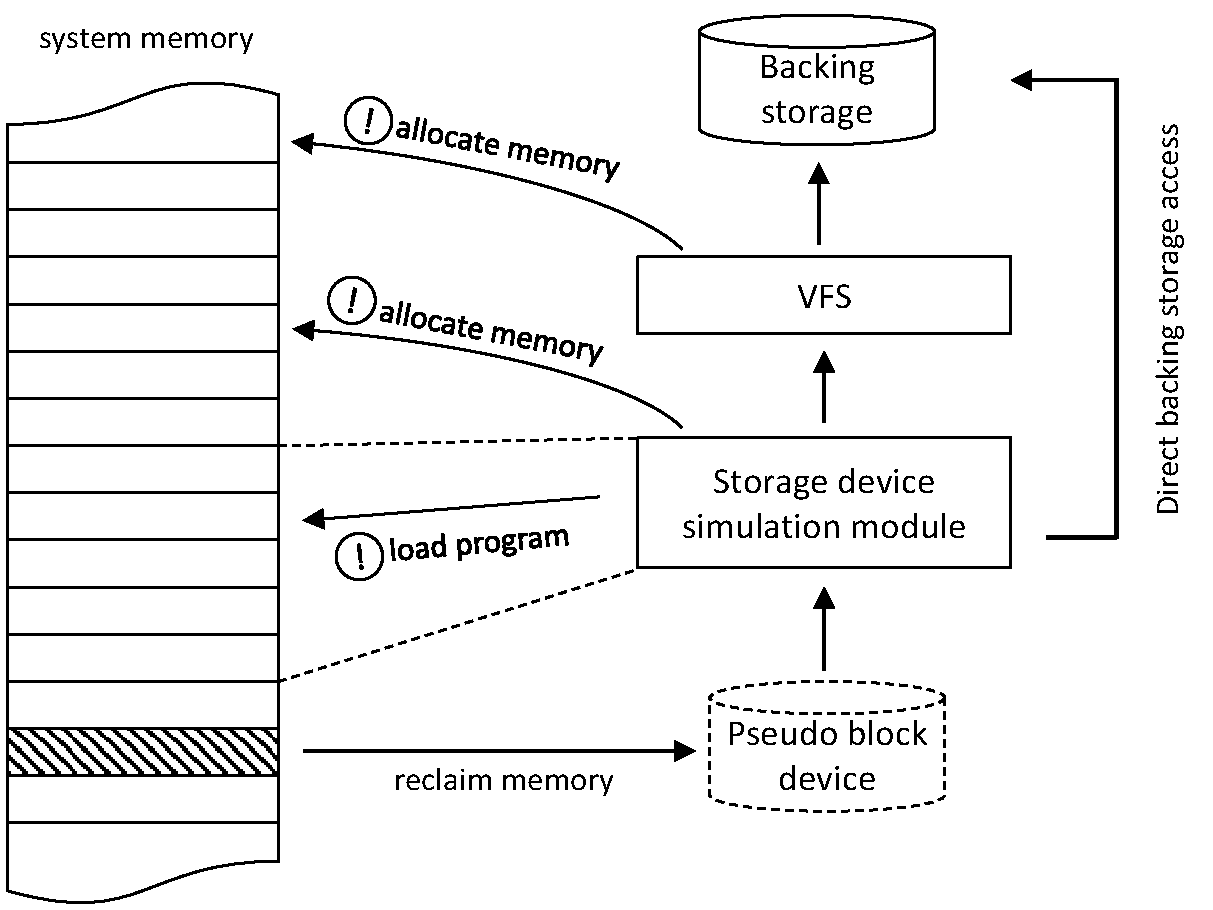
\includegraphics[width=0.8\textwidth]{figures/ch5-direct-backing-storage.pdf}
	\caption{\label{fig:ch5-direct-backing-storage}Avoid allocating memory in the storage device simulation path.}
\end{figure}


\section{Integration with Third-Party Disk Simulators}
\label{sec:disk-simulator-integration}

The storage device simulation module relies on disk simulators to calculate the I/O service timings and simulate the behaviors of the target storage device. The storage device simulation module has three main functions:
\begin{enumerate*}[label=(\arabic*)]
	\item \label{ch5-third-party-one} Calculate the service times of the I/O requests using a disk model, 
	\item \label{ch5-third-party-two} Save and retrieve the actual data of the I/O requests to and from the backing storage, and
	\item \label{ch5-third-party-three} Submit the I/O responses to the Linux kernel at the corresponding service times as calculated in \ref{ch5-third-party-one}.
\end{enumerate*}

The storage device simulation module provides a well-defined API for integration with third-party disk simulators. When third-party disk simulators are integrated into the proposed full-system co-simulator, they can be used by the storage device simulation module to calculate the service timings in \ref{ch5-third-party-one}. Because the designs of \ref{ch5-third-party-two} and \ref{ch5-third-party-three} are decoupled with \ref{ch5-third-party-one}, no additional modifications will be needed if a different disk simulator is used for calculating the service timings of the I/O requests.

\begin{figure}[htpb!]
	\centering
	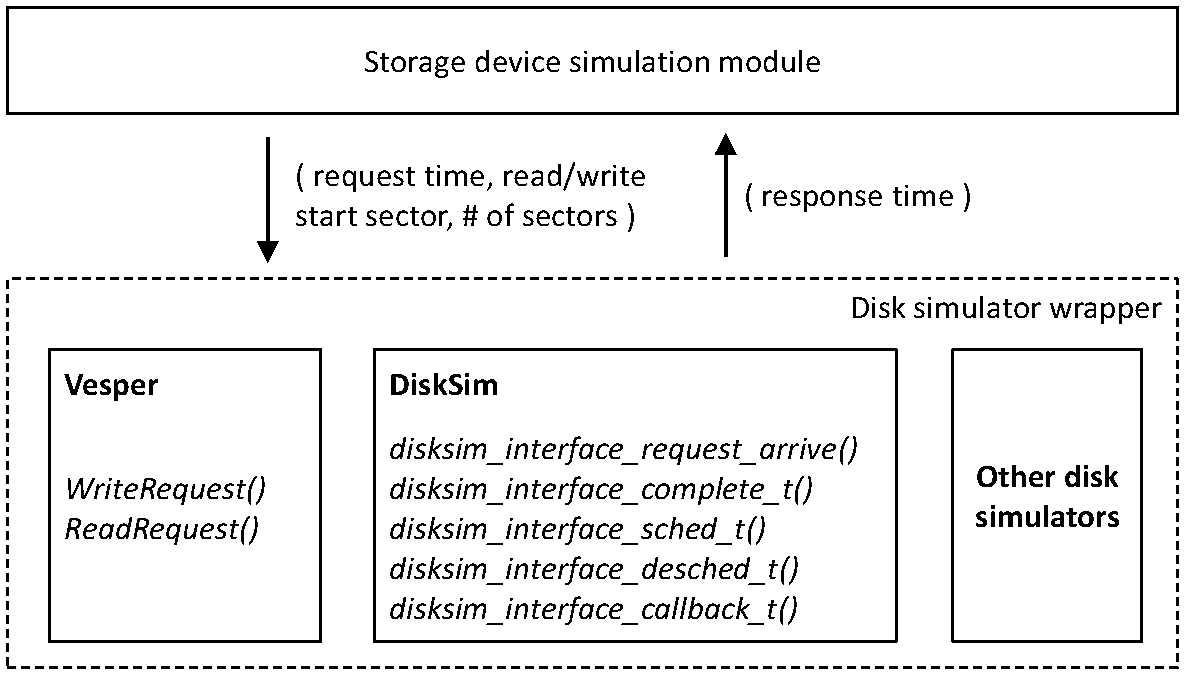
\includegraphics[width=0.85\textwidth]{figures/ch5-disk-simulator-integration.pdf}
	\caption{\label{fig:ch5-disk-simulator-integration}Interface for integration with third-party disk simulators.}
\end{figure}

As illustrated in Figure~\ref{fig:ch5-disk-simulator-integration}, the interface for integrating third-party disk simulators with the storage device simulation module is simple. For each I/O request, the storage device simulation module will provide four pieces of information to the disk simulator: request time, request type (read or write), start sector, and number of sectors. The responsibility of the disk simulator is to calculate the response timings of the I/O requests and return them to the storage device simulation module. If the APIs provided by the third-party disk simulators are different from the aforementioned interface, wrappers can be used for adapting to the provided APIs.

The proposed full-system co-simulator is integrated with two disk simulators: Vesper~\cite{DeRosa:2006} and DiskSim~\cite{Bucy:2008}. The Vesper disk simulator was originally released as part of the Nachos instructional OS~\cite{Christopher:1993}. The source code of Vesper is separated from Nachos~\cite{Pearson:2007} and made operational as a standalone library. A wrapper is developed to make Vesper compatible with the storage device simulation module's API interface. In this case, the wrapper simply uses one of the internal \textit{WriteReqeust} or \textit{ReadRequest} API of Vesper to compute the service timings for the incoming I/O requests.

The second disk simulator that is supported is the DiskSim simulator. DiskSim is itself implemented as a discrete event simulator. It provides APIs for injecting and receiving events from its internal simulation loop. When an I/O request is to be processed, the wrapper injects the I/O request into DiskSim using the \textit{disksim_interface_request_arrive} function. It then simulates DiskSim until the I/O completion time is reported from DiskSim through the \textit{disksim_interface_complete_t} function callback.

\section{Experimental Results}
\label{sec:ch5-experimental-results}
The target platform used for evaluating the proposed full-system co-simulator is a computer equipped with a 3.1 GHz Intel Core i5-3210M processor and 16 GB of DDR3 memory. A 240 GB Intel 520 series SSD is used as the backing storage. The storage device simulation module in the proposed full-system co-simulator supports two different kinds of disk simulators: DiskSim and Vesper. It also supports two types of backing storages: SSD and RAM.

DiskSim provides more detailed simulation of the behaviors of the disk device at the cost of higher computation complexity. Vesper is a faster disk simulator that provides adequate realism for system-level performance evaluations. In some system-level performance studies, very detailed modeling of a specific disk device is not needed. For example, when designing the I/O scheduling algorithm in an OS for general rotational disks, using a disk simulator that captures the essential characteristics of the rotational mechanical disk devices will be sufficient as the I/O scheduling algorithm will be used with different disk devices. In this case, only simulating the essential characteristics of mechanical disk devices such as disk head track switching time, rotational delay, and buffering could be adequate. Vesper can be chosen as the disk simulator when conducting this kind of system-level performance evaluations.

Because the system time of the Linux OS is controlled by the simulation kernel and is no longer linked the real-world clock time, it cannot be used for measuring the elapsed time of the simulation. A special system call is added to the Linux kernel for getting the real wall clock time from the real hardware counter. On the test computer, the Time Stamp Counter (TSC), which is available on all modern x86 processors, is used for measuring the elapsed wall clock time. The TSC counter is incremented every CPU clock cycle. With the CPU running at 3.1GHz on the test computer, the TSC counter has a resolution of approximately 0.3\si{\nano\second}.

For the testing workloads, vdbench (version 5.02)~\cite{Vdbench:2013} is used for generating 18 kinds of I/O access profiles. Each workload profile has three attributes: access type, read/write type, and request size. The access type can be ``random'' or ``mixed.'' The read/write type can be ``read,'' ``write,'' or ``read-write.'' The request size can be ``small,'' ``uniform,'' or ``large.'' A random workload has zero probability of local accesses or sequential accesses; request starting locations are uniformly distributed across the entire storage capacity of the tested hard disk drive. A mixed workload has 80\% probability of random accesses and 20\% of sequential accesses. A read workload is composed of all read accesses, a write workload is composed of all write accesses, and a read-write workload is composed of 50\% read accesses and 50\% write accesses. A small workload is composed of 8-sector (4KB) requests, a large workload uses 256-sector (128KB) requests, and a uniform workload has uniformly distributed request sizes in intervals of 4KB over the range [4KB, 128KB]. All workload profiles continuously generate I/O requests at the maximal speed at which can be sustained by the simulated storage device for 3 minutes.

\subsection{Timing Accuracy of the Simulated Storage Device}

In the work of timing-accurate storage emulation by Griffin et al.~\cite{Griffin:2002}, to evaluate how closely the storage emulator comes to perfect timing-accurate emulation, they have compared the per-request I/O service times observed by the OS to the per-request service times as reported by the DiskSim disk simulator. If the differences between the OS observed I/O service times and the times reported by DiskSim is small, then it means that the performance characteristics of the emulated storage device as perceived by the OS is close to the intended target. From their experimental results, it had been shown that the performance prediction accuracy is good when over 99\% of all emulated I/O responses have less than 2\% error. 

In the proposed full-system co-simulator, when an I/O request is received by the storage device simulation module, it will use the disk simulator (e.g., DiskSim or Vesper) to calculate the intended response time for the I/O request. The storage device simulation module will then register a timer to wait for the arrival of the intended response time. When the timer expires, the storage device simulation module will wake up and reply the I/O response to the Linux kernel. Due to things such as OS state pausing overhead and process context switch latencies, the time point at which the Linux kernel receives the I/O response might not be exactly the same as the intended response time as calculated by the disk simulator. For example, if the disk simulator calculates that an I/O request should be completed at time $t$ and that the Linux kernel actually receives the I/O response at time $t + \Delta t$, then the timing error value of the I/O response is said to be $\Delta t$. The percent timing error of the I/O response is $(\Delta t / t) \times 100\%$. 

The timing error of the simulated storage device in the proposed full-system co-simulator is measured. The storage device simulation module is configured with the Vesper disk simulator and using SSD as the backing storage. The target storage device modeled is the IBM 08K0383 36G hard disk drive. Each of the 18 workload profiles generated by vdbench is submitted to the simulated storage device. The timing errors for a total of 468,964 I/O responses are measured. Figure~\ref{fig:ch5-fig-15a} shows the distribution of the timing error values. Over 99.995\% of the I/O responses measured have a timing error value of less than 20\si{\micro\second}. Figure~\ref{fig:ch5-fig-15b} shows the distribution of the percent timing errors. The percent timing error of an I/O response is calculated by dividing the timing error value by the service time of the corresponding I/O request as computed by the Vesper disk simulator. Over 99.98\% of all the I/O responses measured have less than 0.5\% timing error.

\begin{figure}[htpb]
	\centering
	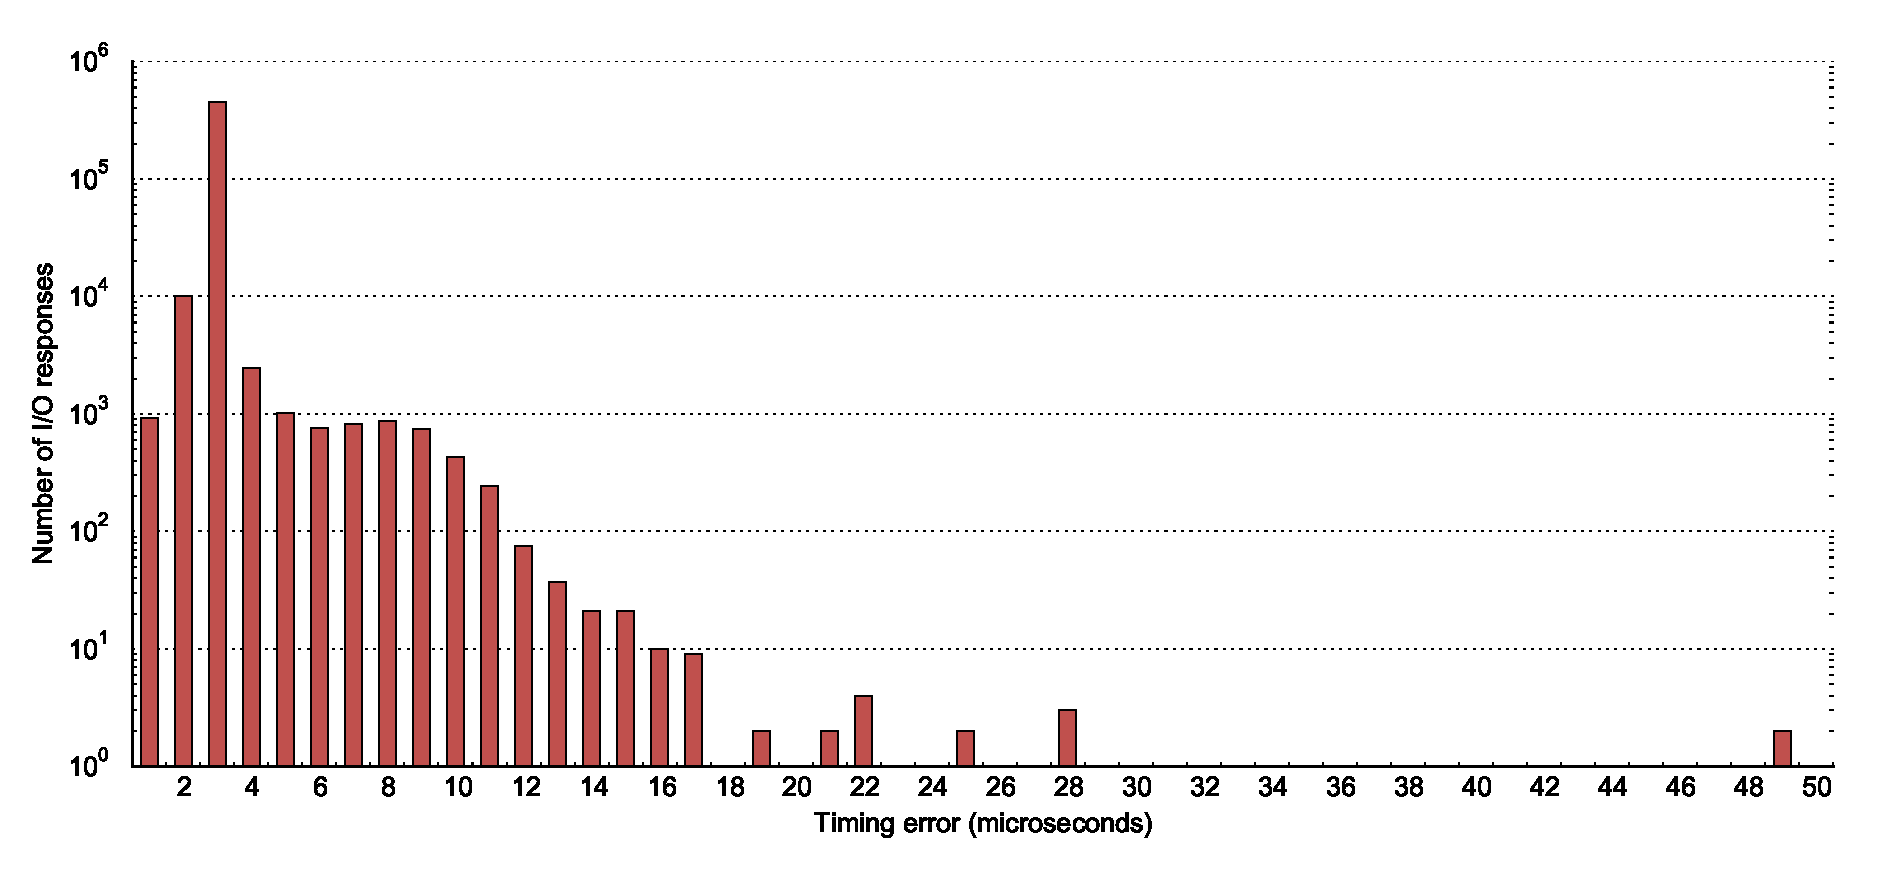
\includegraphics[width=\textwidth]{figures/ch5-fig-15a.pdf}
	\caption{\label{fig:ch5-fig-15a}Timing error of the simulated storage device.}
\end{figure}

\begin{figure}[htpb]
	\centering
	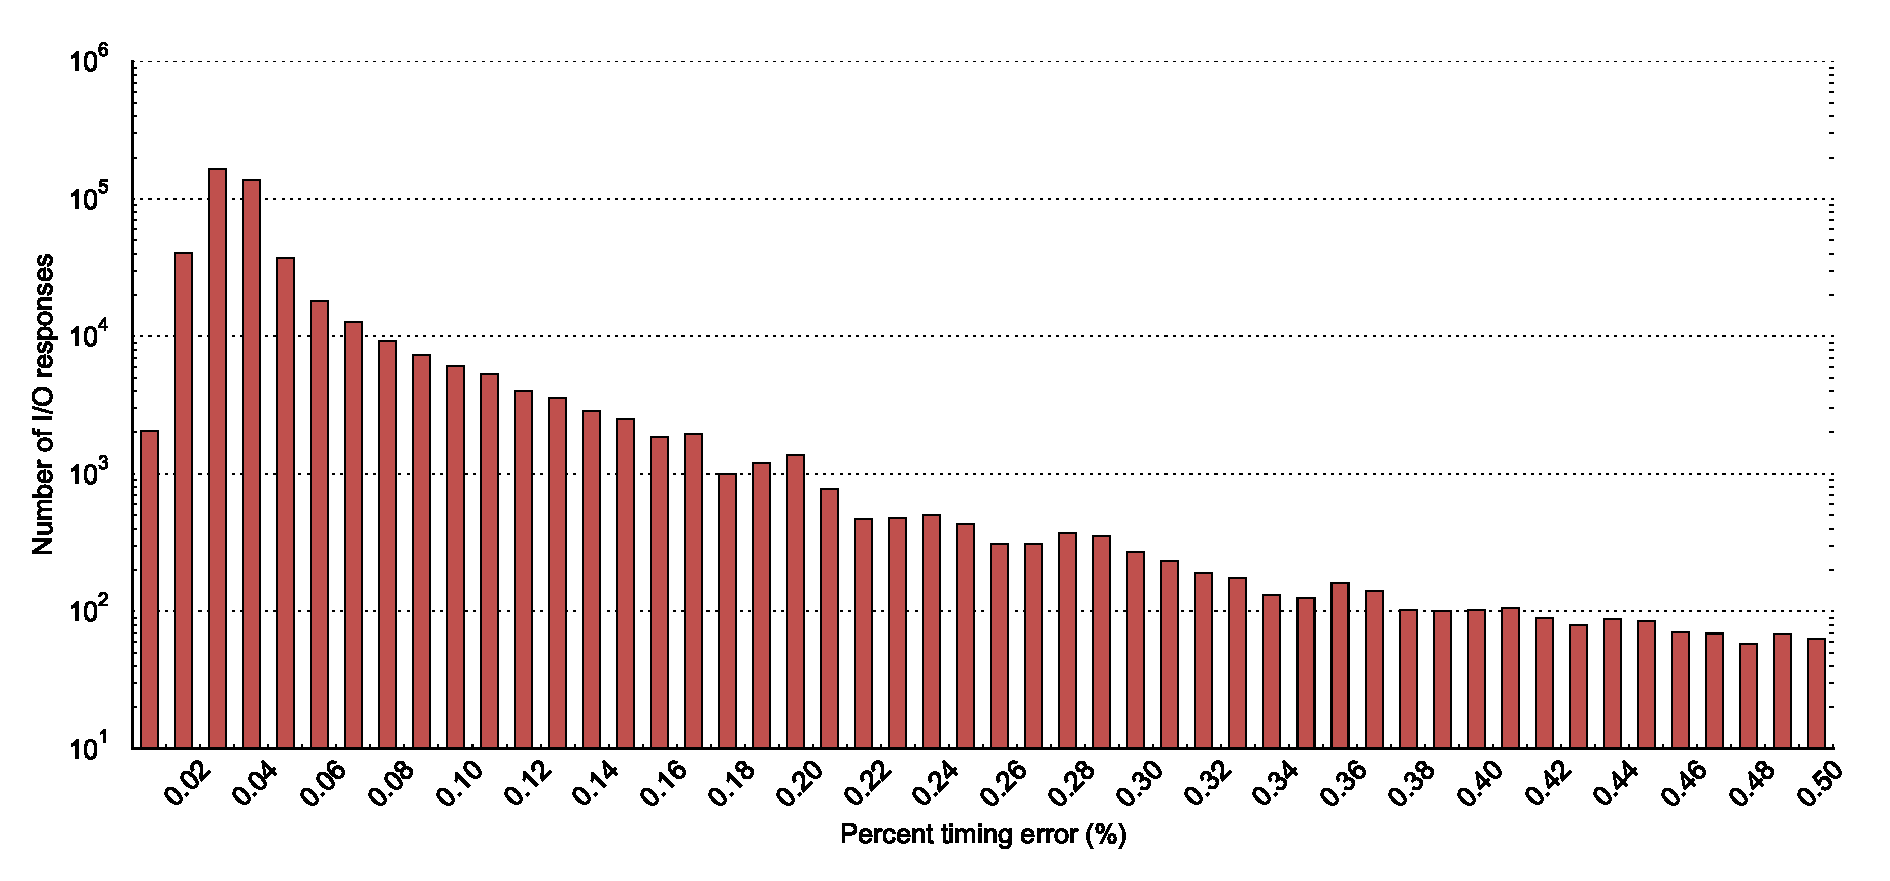
\includegraphics[width=\textwidth]{figures/ch5-fig-15b.pdf}
	\caption{\label{fig:ch5-fig-15b}Percent timing error of the simulated storage device.}
\end{figure}


\subsection{Simulation Speed}
\label{sec:simulation-performance}

The speed at which the proposed full-system co-simulator can carry out the simulation process depends on many factors. The three most relevant factors are summarized as follows:

\begin{itemize}
	\item The performance of the simulate storage device that is modeled --- The faster the simulated storage device is, the more I/O requests can be handled during the same system time span, and thus the more simulation work needs to be carried out. For example, when the storage subsystem is fully stressed, simulating a system equipped with a 15k RPM disk will be slower than simulating the same system equipped with a 5.4k RPM disk.
	
	\item The performance of the storage device simulation module --- The faster the storage device simulation module can compute the I/O request timings and handle the actual data of the simulated storage device, the faster the simulation process will be. Therefore, using a simple disk model simulator such as Vesper will be faster than using a more complex disk model simulator such as DiskSim. Similarly, using RAM as the backing storage will be faster than using a storage device as the backing storage.
	
	\item The I/O access pattern of the benchmark workload --- Different benchmark workload will generate I/O requests of different intensity. A light weight benchmark workload will leave the co-simulator more time in the CPU idle loop. This means that there will be more opportunity for time-skipping the CPU idle loop and thus leads to faster simulation speed.
\end{itemize}

Table~\ref{tab:DiskSim-and-SSD-result} to Table~\ref{tab:Vesper-and-RAM-speed} show the experimental results. The meaning of the columns in the tables are explained as follows. The ``Simulation result'' columns show the metrics measured on the Linux OS, which are respect to the virtual time system. ``I/O per second'' and ``Bandwidth'' are the benchmark results from the vdbench program. ``Elapsed system time'' is the time span that vdbench is running and generating workloads toward the simulated storage device. It is measured using the \textit{time} command of the Linux OS. The values in the ``vdbench CPU time'' column are also measured using the \textit{time} command, showing the user and system CPU time used by vdbench. The values in the ``Simulation speed'' columns are measured using the real TSC clock. ``Elapsed wall clock time'' is the total amount of time that the proposed full-system co-simulator used for carrying out the simulation. The ``In paused mode'' column shows how much time the Linux OS is put into the ``paused'' mode. The ``DiskSim busy'' or the ``Vesper busy'' column shows how much time when the OS in the ``paused'' mode is consumed by DiskSim or Vesper. The ``Backing storage busy'' column shows how much time during the simulation is spent waiting for the backing storage. The final column shows the speedup that the proposed full-system co-simulator has achieved. The values in this column equal to the ratio between the values of ``Elapsed system time'' and ``Elapsed wall clock time''.

In the first set of experiments, DiskSim is configured as the disk simulator and SSD is used as the backing storage. The virtual storage device being simulated is a Seagate Cheetah 15k.5 147GB hard disk drive. It has a spindle speed of 15K and an average seek time of less than 4\si{\milli\second}. The raw disk device is benchmarked. The device is opened with the O_DIRECT flag to bypass the system buffer caches. The experimental results are shown in Table~\ref{tab:DiskSim-and-SSD-result} and Table~\ref{tab:DiskSim-and-SSD-speed}. For each simulation run, the system is rebooted to prevent interferences from the previous executions. Observations from the first set of experimental results are summarized as follows.

\begin{itemize}
	\item The proposed full-system co-simulator has achieved faster-than-real-time simulation of a complete system running the Linux OS with DiskSim simulating a modern server grade hard disk drive. The speedup achieved in the experimental setup is between 1.07$\times$ to 2.27$\times$.
	
	\item Because vdbench is an I/O bound benchmark application, not much CPU time is consumed by vdbench. During the simulated time span, the Linux OS is relatively idle and can be time skipped. Note that when the values in ``Time used by vdbench'' is subtracted from  the values in ``Simulated timespan'', the resulting numbers are very close to the total simulation time that can be time skipped.
	
	\item The majority of the simulation time is consumed by DiskSim. Over 97\% of the time when the OS is in the paused mode is used by DiskSim.
	
	\item For each test, the summation of the value in the ``DiskSim computation time'' column and the value in the ``Backing storage operation time'' column can be longer than the total time spent in the paused mode. This is because the design of the storage simulation module allows backing storage to work in parallel while the request timings are being calculated.
\end{itemize}

\begin{table}[htbp]%
\small
\begin{center}
\caption{Simulation results for DiskSim and SSD}\label{tab:DiskSim-and-SSD-result}
\hspace*{-2cm}
\noindent\begin{tabular}{lcS[table-format=2.2]cc}
	\toprule
	& \multicolumn{4}{c}{Simulation result} \\
	\cmidrule(lr){2-5}
	\parbox{3cm}{\centering Workload \\ profile} & \parbox{2cm}{\centering I/O per \\ second } & \parbox{2cm}{\centering Bandwidth \\ (MB/sec) } & \parbox{2cm}{\centering Elapsed \\ system time} & \parbox{3cm}{\centering vdbench CPU time\\ (user / sys)} \\
	
	\midrule
	
	random / read / small & 172.75 & 0.67 & 187.945 & 2.416 / 0.082 \\
	random / read / large &	140.74 & 17.59 & 187.305 & 2.444 / 0.960 \\
	random / read / uniform & 155.06 & 10.01 & 188.285 & 2.344 / 0.904 \\
	random / write / small & 171.51 & 0.67 & 187.495 & 2.540 / 0.900 \\
	random / write / large & 142.76 & 17.84 & 188.986 & 2.432 / 1.144 \\
	random / write / uniform & 156.09 & 10.07 & 187.574 & 2.760 / 0.872 \\
	random / read-write / small & 170.45 & 0.67 & 187.277 & 2.604 / 0.760 \\
	random / read-write / large & 140.15 & 17.52 & 188.050 & 2.468 / 1.032 \\
	random / read-write / uniform & 153.99 & 9.95 & 188.448 & 2.524 / 0.920 \\
	mixed / read / small & 243.19 & 0.95 & 189.274 & 2.344 / 1.040 \\
	mixed / read / large & 186.37 & 23.30 & 187.214 & 2.592 / 1.184 \\
	mixed / read / uniform & 211.22 & 13.67 & 187.741 & 2.540 / 1.120 \\
	mixed / write / small & 195.20 & 0.76 & 187.818 & 2.620 / 0.944 \\
	mixed / write / large & 160.27 & 20.03 & 190.912 & 2.556 / 1.188 \\
	mixed / write / uniform & 176.60 & 11.43 & 187.470 & 2.708 / 1.164 \\
	mixed / read-write / small & 210.87 & 0.82 & 187.173 & 2.648 / 0.908 \\
	mixed / read-write / large & 169.69 & 21.21 & 188.417 & 2.584 / 1.196 \\
	mixed / read-write / uniform & 188.50 & 12.23 & 187.386 & 2.676 / 1.080 \\

	\bottomrule
\end{tabular}
\hspace*{-2cm}
\end{center}

	Remarks: The full-system co-simulator is configured to use DiskSim as the disk simulator and SSD as the backing storage. The target storage device modeled is the 147GB Seagate Cheetah 15k.5 hard disk drive. Units are in seconds unless otherwise specified.
\end{table}%


\begin{table}[htbp]%
	\small
	\begin{center}
	\caption{Simulation speed for DiskSim and SSD}\label{tab:DiskSim-and-SSD-speed}
	\hspace*{-2cm}
	\noindent\begin{tabular}{
			l
			S[table-format=3.3]
			S[table-format=3.3]
			r
			S[table-format=3.3]
			c
			}
		\toprule
		& \multicolumn{5}{c}{Simulation speed} \\
		\cmidrule(lr){2-6}
		\parbox{3cm}{\centering Workload \\ profile} & \parbox{1.8cm}{\centering Elapsed \\ wall clock \\ time } & \parbox{1.2cm}{\centering In paused mode } & \parbox{3.2cm}{\centering DiskSim busy \\ (\% of paused mode)} & \parbox{1.2cm}{\centering Backing \\ storage \\ busy} & \parbox{1.5cm}{\centering Speedup \\ over \\ real-time}\\
		
		\midrule
		
		random / read / small & 82.659 & 78.746 & 77.246 (98.09\%) & 8.165 & 2.27$\times$ \\
		random / read / large &	140.425 & 136.388 & 134.363 (98.52\%) & 54.385 & 1.33$\times$ \\
		random / read / uniform & 116.217 & 112.315 & 110.462 (98.35\%) & 34.336 & 1.62$\times$ \\
		random / write / small & 79.065 & 74.878 & 73.410 (98.04\%) & 8.970 & 2.37$\times$ \\
		random / write / large & 145.042 & 140.651 & 138.142 (98.22\%) & 95.977 & 1.30$\times$ \\
		random / write / uniform & 115.682 & 111.270 & 109.209 (98.15\%) & 55.715 & 1.62$\times$ \\
		random / read-write / small & 79.163 & 75.071 & 73.747 (98.24\%) & 8.526 & 2.37$\times$ \\
		random / read-write / large & 141.414 & 137.181 & 135.054 (98.45\%) & 73.220 & 1.33$\times$ \\
		random / read-write / uniform & 116.484 & 112.294 & 110.444 (98.35\%) & 45.032 & 1.62$\times$ \\
		mixed / read / small & 86.378 & 82.221 & 80.369 (97.75\%) & 8.791 & 2.19$\times$ \\
		mixed / read / large & 165.248 & 160.728 & 158.086 (98.36\%) & 70.891 & 1.13$\times$ \\
		mixed / read / uniform & 129.401 & 124.952 & 122.480 (98.02\%) & 44.712 & 1.45$\times$ \\
		mixed / write / small & 119.795 & 115.464 & 113.844 (98.60\%) & 8.259 & 1.57$\times$ \\
		mixed / write / large & 178.576 & 173.933 & 171.083 (98.36\%) & 105.511 & 1.07$\times$ \\
		mixed / write / uniform & 153.308 & 148.564 & 146.152 (98.38\%) & 61.404 & 1.22$\times$ \\
		mixed / read-write / small & 106.426 & 102.080 & 100.494 (98.45\%) & 8.557 & 1.76$\times$ \\
		mixed / read-write / large & 171.517 & 166.913 & 164.363 (98.47\%) & 87.658 & 1.10$\times$ \\
		mixed / read-write / uniform & 141.370 & 136.767 & 134.503 (98.34\%) & 52.583 & 1.33$\times$ \\
		
		\bottomrule
	\end{tabular}
	\hspace*{-2cm}
	\end{center}

	Remarks: The full-system co-simulator is configured to use DiskSim as the disk simulator and SSD as the backing storage. The target storage device modeled is the 147GB Seagate Cheetah 15k.5 hard disk drive. Units are in seconds unless otherwise specified.
\end{table}%

In the second set of experiments, the proposed full-system co-simulator is configured to use Vesper as the disk simulator for calculating the service timings of the simulated storage device. The disk profile for the IBM 08K0383 36GB disk drive that comes with Vesper is used as the disk model for the simulated storage device. The IBM disk drive has a spindle speed of 10K and an average seek time of 4.7ms. The experimental results are shown in Table~\ref{tab:Vesper-and-SSD-result} and Table~\ref{tab:Vesper-and-SSD-speed}. Only the results for the ``mixed'' set of workload profiles are shown. Observations from the experimental results are summarized as follows.

\begin{itemize}
	\item Due to its simplicity, Vesper can calculate response timings for the simulated disk device much faster than DiskSim. Our measurements show that Vesper is up to three orders of magnitude faster than DiskSim.
	
	\item The backing storage operation is now dominating the time that the proposed full-system co-simulator spends in the paused mode. This leads to the motivation of the next set of experiments, which uses RAM as the backing storage to further speedup the simulation speed.
\end{itemize}

In the third set of experiments, the proposed full-system co-simulator uses Vesper for storage device timing calculation and RAM as the backing storage device. The IBM 08K0383 36GB disk drive is modeled. The experimental results are shown in Table~\ref{tab:Vesper-and-RAM-result} and Table~\ref{tab:Vesper-and-RAM-speed}. Only the results for the ``mixed'' set of workload profiles are shown. Some observations are:

\begin{itemize}
	\item Only a small fraction of time is now used by Vesper and the RAM-based backing storage. The proposed full-system co-simulator consistently achieves simulation speed of over 30$\times$ to 45$\times$ faster than real-time.
	
	\item Vdbench and other housekeeping tasks in the proposed full-system co-simulator are now accounting for over 90\% of the simulation time. By Amdahl's law, switching to an even faster disk timing simulator or backing storage will not have much gain for the simulation speed.
\end{itemize}

In summary, it has been demonstrated that the overhead of the proposed full-system co-simulator itself is lightweight and can achieve a full-system simulation speed of over 45 times faster than real-time in real world usage scenarios.

\begin{table}[htbp]%
	\small
	\begin{center}
	\caption{Simulation results for Vesper and SSD}\label{tab:Vesper-and-SSD-result}
	\hspace*{-2cm}
	\noindent\begin{tabular}{lS[table-format=3.2]ccc}
		\toprule
		& \multicolumn{4}{c}{Simulation result} \\
		\cmidrule(lr){2-5}
		\parbox{3cm}{\centering Workload \\ profile} & \parbox{2cm}{\centering I/O per \\ second } & \parbox{2cm}{\centering Bandwidth \\ (MB/sec) } & \parbox{2cm}{\centering Elapsed \\ system time} & \parbox{3cm}{\centering vdbench CPU time\\ (user / sys)} \\
		
		\midrule
		
		mixed / read / small & 147.28 & 0.58 & 186.337 & 2.364 / 0.652 \\
		mixed / read / large & 73.93 & 9.24 & 186.866 & 2.496 / 0.768 \\
		mixed / read / uniform & 97.96 & 6.33 & 187.867 & 2.452 / 0.688 \\
		mixed / write / small & 147.62 & 0.58 & 186.853 & 2.508 / 0.836 \\
		mixed / write / large & 73.79 & 9.22 & 187.346 & 2.504 / 0.944 \\
		mixed / write / uniform & 97.92 & 6.33 & 186.375 & 2.708 / 0.812 \\
		mixed / read-write / small & 146.84 & 0.57 & 185.886 & 2.428 / 0.744 \\
		mixed / read-write / large & 73.76 & 9.22 & 186.842 & 2.376 / 0.752 \\
		mixed / read-write / uniform & 97.91 & 6.37 & 186.874 & 2.528 / 0.796 \\
		
		\bottomrule
	\end{tabular}
	\hspace*{-2cm}
	\end{center}

	Remarks: The full-system co-simulator is configured to use Vesper as the disk simulator and SSD as the backing storage. The target device modeled is the 36GB IBM 08K0383 hard disk drive. Units are in seconds unless otherwise specified.
\end{table}%


\begin{table}[htbp]%
	\small
	\begin{center}
	\caption{Simulation speed for Vesper and SSD}\label{tab:Vesper-and-SSD-speed}
	\hspace*{-2cm}
	\noindent\begin{tabular}{
			l
			S[table-format=2.3]
			S[table-format=2.3]
			c
			S[table-format=2.3]
			S[table-format=2.2]
			}
		\toprule
		& \multicolumn{5}{c}{Simulation speed} \\
		\cmidrule(lr){2-6}
		\parbox{3cm}{\centering Workload \\ profile} & \parbox{1.8cm}{\centering Elapsed \\ wall clock \\ time } & \parbox{1.2cm}{\centering In paused mode } & \parbox{3.2cm}{\centering DiskSim busy \\ (\% of paused mode)} & \parbox{1.2cm}{\centering Backing \\ storage \\ busy} & \parbox{1.5cm}{\centering Speedup \\ over \\ real-time}\\
		
		\midrule
		
		mixed / read / small & 6.358 & 2.585 & 0.053 (2.04\%) & 3.819 & 29.31$\times$ \\
		mixed / read / large & 24.512 & 20.351 & 0.052 (0.25\%) & 22.071 & 7.62$\times$ \\
		mixed / read / uniform & 22.331 & 18.399 & 0.043 (0.23\%) & 19.932 & 8.41$\times$ \\
		mixed / write / small & 8.335 & 4.193 & 0.047 (1.12\%) & 5.552 & 22.42$\times$ \\
		mixed / write / large & 49.633 & 45.195 & 0.038 (0.08\%) & 47.577 & 3.77$\times$ \\
		mixed / write / uniform & 36.520 & 32.082 & 0.040 (0.12\%) & 34.131 & 5.10$\times$ \\
		mixed / read-write / small & 8.159 & 4.236 & 0.052 (1.23\%) & 5.515 & 22.78$\times$ \\
		mixed / read-write / large & 39.853 & 35.904 & 0.063 (0.18\%) & 37.872 & 4.69$\times$ \\
		mixed / read-write / uniform & 29.906 & 25.739 & 0.047 (0.18\%) & 27.499 & 6.25$\times$ \\
		
		\bottomrule
	\end{tabular}
	\hspace*{-2cm}
	\end{center}

	Remarks: The full-system co-simulator is configured to use Vesper as the disk simulator and SSD as the backing storage. The target device modeled is the 36GB IBM 08K0383 hard disk drive. Units are in seconds unless otherwise specified.
\end{table}%


% -------------------------- Vesper and RAM

\begin{table}[htbp]%
	\small
	\begin{center}
	\caption{Simulation results for Vesper and RAM}\label{tab:Vesper-and-RAM-result}
	\hspace*{-2cm}
	\noindent\begin{tabular}{lS[table-format=3.2]ccc}
		\toprule
		& \multicolumn{4}{c}{Simulation result} \\
		\cmidrule(lr){2-5}
		\parbox{3cm}{\centering Workload \\ profile} & \parbox{2cm}{\centering I/O per \\ second } & \parbox{2cm}{\centering Bandwidth \\ (MB/sec) } & \parbox{2cm}{\centering Elapsed \\ system time} & \parbox{3cm}{\centering vdbench CPU time\\ (user / sys)} \\
		
		\midrule
		
		mixed / read / small & 146.79 & 0.57 & 186.330 & 2.228 / 0.532 \\
		mixed / read / large & 73.83 & 9.23 & 188.614 & 2.420 / 0.504 \\
		mixed / read / uniform & 97.60 & 6.30 & 186.335 & 2.368 / 0.560 \\
		mixed / write / small & 147.51 & 0.58 & 186.387 & 2.668 / 0.540 \\
		mixed / write / large & 73.88 & 9.24 & 188.355 & 2.568 / 0.576 \\
		mixed / write / uniform & 97.95 & 6.33 & 187.117 & 2.852 / 0.540 \\
		mixed / read-write / small & 147.81 & 0.58 & 186.830 & 2.388 / 0.496 \\
		mixed / read-write / large & 73.82 & 9.23 & 188.101 & 2.640 / 0.572 \\
		mixed / read-write / uniform & 97.84 & 6.37 & 186.942 & 2.564 / 0.528 \\
		
		\bottomrule
	\end{tabular}
	\hspace*{-2cm}
	\end{center}

	Remarks: The full-system co-simulator is configured to use Vesper as the disk simulator and RAM as the backing storage. The target device modeled is the 36GB IBM 08K0383 hard disk drive. Units are in seconds unless otherwise specified.
\end{table}%


\begin{table}[htbp]%
	\small
	\begin{center}
	\caption{Simulation speed for Vesper and RAM}\label{tab:Vesper-and-RAM-speed}
	\hspace*{-2cm}
	\noindent\begin{tabular}{lccccc}
		\toprule
		& \multicolumn{5}{c}{Simulation speed} \\
		\cmidrule(lr){2-6}
		\parbox{3cm}{\centering Workload \\ profile} & \parbox{1.8cm}{\centering Elapsed \\ wall clock \\ time } & \parbox{1.2cm}{\centering In paused mode } & \parbox{3.2cm}{\centering DiskSim busy \\ (\% of paused mode)} & \parbox{1.2cm}{\centering Backing \\ storage \\ busy} & \parbox{1.5cm}{\centering Speedup \\ over \\ real-time}\\
		
		\midrule
		
		mixed / read / small & 4.052 & 0.689 & 0.036 (5.23\%) & 0.060 & 45.99$\times$ \\
		mixed / read / large & 5.117 & 1.618 & 0.033 (2.02\%) & 0.779 & 36.86$\times$ \\
		mixed / read / uniform & 4.784 & 1.283 & 0.034 (2.66\%) & 0.534 & 38.95$\times$ \\
		mixed / write / small & 4.562 & 0.727 & 0.035 (4.80\%) & 0.091 & 40.85$\times$ \\
		mixed / write / large & 5.941 & 2.188 & 0.031 (1.41\%) & 1.265 & 31.70$\times$ \\
		mixed / write / uniform & 5.691 & 1.683 & 0.033 (1.94\%) & 0.866 & 32.88$\times$ \\
		mixed / read-write / small & 4.214 & 0.719 & 0.036 (5.06\%) & 0.076 & 44.33$\times$ \\
		mixed / read-write / large & 5.712 & 1.900 & 0.033 (1.75\%) & 1.025 & 32.93$\times$ \\
		mixed / read-write / uniform & 5.254 & 1.500 & 0.034 (2.28\%) & 0.711 & 35.58$\times$\\
		
		\bottomrule
	\end{tabular} 
	\hspace*{-2cm}
	\end{center}

	Remarks: The full-system co-simulator is configured to use Vesper as the disk simulator and RAM as the backing storage. The target device modeled is the 36GB IBM 08K0383 hard disk drive. Units are in seconds unless otherwise specified.
\end{table}%


\section{Applications of the Proposed Full-System Co-Simulator}
\label{sec:use-case}

Using the proposed full-system co-simulator, virtually simulated storage device can be co-simulated with the real OS and application programs running on the physical computer hardware. This means that realistic real-world workloads and system-level measurement metrics can be used for predicting the performance of the simulated storage device. Sections~\ref{sec:ch5-faster-storage-devices} and \ref{sec:ch5-different-CPU-speeds} describes two example applications of the proposed full-system co-simulator.

\subsection{Studying the Effects of Having Faster Storage Devices}
\label{sec:ch5-faster-storage-devices}

The proposed full-system co-simulator can simulate storage devices that are faster and larger than the actual storage device available. This allows system-level effects to be studied assuming when storage devices of different speeds are available. During simulation, the state of the Linux OS can be paused to wait for the storage device simulation module to process the I/O requests. Therefore, the amount of time used for preparing the I/O responses will not affect the storage device's performance as perceived by the Linux OS. For example, even if the storage device simulation module uses 100\si{\milli\second} to prepare for the response of an I/O request that is supposed to have a service time of 10\si{\milli\second} to the OS, due to the OS state pausing technique, the Linux OS will still perceive that it only took the virtual storage device 10\si{\milli\second} for servicing the I/O request. This allows the proposed co-simulation environment to simulate storage devices that are faster than the real backing storage that is available.

When the real data of the simulated storage device is to be saved to the backing storage, a logical-to-physical mapping table is used for data block placement. Data block on the backing storage only needs to be allocated for sectors of the simulated storage device that have been written. This allocation-on-write design allows the proposed full-system co-simulator to simulate storage devices that are larger than the physical backing storage available on the simulation platform if not all sectors of the virtual storage device are written during the benchmarking.

In this section, the proposed full-system co-simulator is used for studying the effects of what faster storage devices will have on the target system. The setup of the target system is the same as described in section~\ref{sec:ch5-experimental-results}. Vesper is used as the disk simulator and the IBM 08K0383 36GB hard disk drive is used as the reference hard disk drive. The performance of the reference disk drive is used as the baseline for modeling other devices. For example, a disk drive marked with 10$\times$ speed should have 10 times the performance of the reference disk drive~\cite{Ruemmler:1994}. The disk configurations that have been studied range from 10$\times$ to 100$\times$ with a stepping of 10$\times$, and from 120$\times$ to 200$\times$ with a stepping of 20$\times$.

In Vesper, the total service time of an I/O request includes the seek time, the rotational delay, and the data transfer time. A simple track cache is also modeled. If the disk head has passed the requested sector after landing at the current track, the read request can be serviced directly by the track cache. The disk models used by Vesper are modeled by its rotational speed, seek times, and data transfer rates. The required seek times are different for different seek distances. The data transfer rates are different from inner to outer tracks. To model a disk drive with 10$\times$ speed in Vesper, the rotational speed and the data transfer rates of the reference disk drive is multiplied by 10, and the seek times are divided by 10.

The metric used for measuring the performance of the system is the amount of time that it takes to extract the bzip2-compressed source archive of the Linux kernel version 3.0.81 (linux-3.0.81.tar.bz2, 74MBytes)~\cite{Kernel:2013}. The archive is extracted to an ext3 file system. The file system is recreated for each test run. The file system is mounted with the sync option so that all writes to the file system are immediately written to the disk. Without setting the sync option, the benchmark could be testing against the caching performance of the system instead of the performance of the simulated disk drive. Two kinds of I/O schedulers are tested. They are the Completely Fair Queuing (CFQ) I/O scheduler~\cite{wiki:2013:CFQ} and the NOOP I/O scheduler~\cite{wiki:2015:NOOP}. The NOOP scheduler is a simple scheduler that only merges I/O requests but does not try to reorder them.

The simulation results for the NOOP scheduler are shown in Table~\ref{tab:ch5-NOOP-scheduler}. The results for the CFQ I/O scheduler are shown in Table~\ref{tab:ch5-CFQ-scheduler}. For both tables, the ``extraction time'' is the simulated extraction time predicted by the proposed full-system co-simulator. The ``ideal extraction time'' is the expected extraction time when assuming that the overall system performance scales linearly with the disk speed. Figure~\ref{fig:ch5-predicted-extraction-time} visualizes the results in the ``extraction time'' column. Figure~\ref{fig:ch5-speedup-over-reference} visualizes the results in the ``speedup over the reference disk'' column.

From ~\ref{fig:ch5-predicted-extraction-time}, observe that the actual extraction performance in both the NOOP and CFQ I/O schedulers are considerably lower than the ideal performance (based on na\"{\i}ve linear-speedup scaling). Looking at the CPU utilization column in Table~\ref{tab:ch5-NOOP-scheduler} and~\ref{tab:ch5-CFQ-scheduler}, notice that the CPU is becoming more utilized as the speed of the disk is raised. This explains the reason why the overall system performance does not scale linearly with the disk speeds. As the performance of the disk is increased, the extraction task is changing from an I/O-bound workload to a CPU-bound workload. Therefore, the CPU is becoming the dominating factor that limits the overall system performance.

Another observation is that when the CFQ scheduler is used, the extraction performance saturates more quickly than when the NOOP scheduler is used. A first guess might be that the CFQ scheduler is more CPU hungry than the NOOP scheduler. However, the CPU utilization rates have never reached over $56\%$ even in the case when the disk speed is $200\times$. Further investigation leads to the \textit{/sys\slash block\slash <device>\slash queue\slash iosched\slash slice_idle} % use \slash to allow line break
parameter of the CFQ scheduler. This parameter controls the amount of time that the CFQ scheduler will intentionally wait for future synchronous requests from different processes, even when there are pending asynchronous requests~\cite{Layton:2009}. The motivation of this design is to favor synchronous requests over asynchronous requests, and it can be viewed as a variant of the anticipatory scheduling algorithm~\cite{Iyer:2001}. The default value of the \textit{slic_idle} parameter is 8\si{\milli\second}. During this waiting period, the CFQ scheduler will not issue asynchronous requests to the storage device. However, in some cases such as when the underlying storage device is very fast, this design can have an adverse effect to the overall system performance.

In the test scenarios, changing the \textit{slice_idle} parameter to 0\si{\milli\second} makes the CFQ scheduler perform comparably to the NOOP scheduler. As we can see, when studying the performance of storage subsystem designs, this kind of complex interactions among the system components can be overlooked if detailed full-system models are not incorporated.

\begin{table}[htbp]%
	\small
	\centering
	\caption{Simulation results for the NOOP scheduler}\label{tab:ch5-NOOP-scheduler}
	\noindent\begin{tabular}{cSSSS}
		\toprule
		\parbox{2cm}{\centering Disk speed} & \parbox{3.5cm}{\centering Predicted extraction \\ time (seconds)} & \parbox{2.5cm}{\centering Speedup over \\ reference disk} & \parbox{3cm}{\centering Ideal extraction \\ time (seconds)} & \parbox{2.5cm}{\centering CPU utilization \\ (\% busy)} \\
		\midrule
		
		1$\times$ (reference) & 1821.706 & 1.00 & \multicolumn{1}{c}{-} & 2.99 \\
		10$\times$ & 214.287 & 8.50 & 1821.71 & 24.92 \\
		20$\times$ & 137.064 & 13.29 & 182.17 & 39.80 \\
		30$\times$ & 83.911 & 21.71 & 91.09 & 59.10 \\
		40$\times$ & 78.298 & 23.27 & 60.72 & 60.46 \\
		50$\times$ & 66.666 & 27.33 & 45.54 & 62.70 \\
		60$\times$ & 50.580 & 36.02 & 36.43 & 69.29 \\
		70$\times$ & 49.169 & 37.05 & 30.36 & 69.76 \\
		80$\times$ & 43.451 & 41.93 & 26.02 & 75.60 \\
		90$\times$ & 37.113 & 49.09 & 22.77 & 86.23 \\
		100$\times$ & 37.949 & 48.00 & 20.24 & 83.43 \\
		120$\times$ & 34.670 & 52.54 & 18.22 & 92.12 \\
		140$\times$ & 37.269 & 48.88 & 15.18 & 95.77 \\
		160$\times$ & 33.692 & 54.07 & 13.01 & 96.36 \\
		180$\times$ & 34.360 & 53.02 & 11.39 & 95.85 \\
		200$\times$ & 30.312 & 60.10 & 10.12 & 97.44 \\
		
		\bottomrule
	\end{tabular}
\end{table}%

\begin{table}[htbp]%
	\small
	\centering
		\caption{Simulation results for the CFQ scheduler}\label{tab:ch5-CFQ-scheduler}
	\noindent\begin{tabular}{cSSSS}
		\toprule
		\parbox{2cm}{\centering Disk speed} & \parbox{3.5cm}{\centering Predicted extraction \\ time (seconds)} & \parbox{2.5cm}{\centering Speedup over \\ reference disk} & \parbox{3cm}{\centering Ideal extraction \\ time (seconds)} & \parbox{2.5cm}{\centering CPU utilization \\ (\% busy)} \\
		\midrule
		
		1$\times$ (reference) & 1968.493 & 1.00 & \multicolumn{1}{c}{-} & 2.91 \\
		10$\times$ & 232.285 & 8.47 & 196.85 & 24.03 \\
		20$\times$ & 157.455 & 12.50 & 98.42 & 35.18 \\
		30$\times$ & 124.959 & 15.75 & 65.62 & 43.09 \\
		40$\times$ & 111.831 & 17.60 & 49.21 & 46.56 \\
		50$\times$ & 100.979 & 19.49 & 39.37 & 49.19 \\
		60$\times$ & 96.806 & 20.33 & 32.81 & 51.66 \\
		70$\times$ & 92.814 & 21.21 & 28.12 & 51.01 \\
		80$\times$ & 93.545 & 21.04 & 24.61 & 52.71 \\
		90$\times$ & 86.753 & 22.69 & 21.87 & 52.93 \\
		100$\times$ & 88.153 & 22.33 & 19.68 & 53.64 \\
		120$\times$ & 84.121 & 23.40 & 16.40 & 54.43 \\
		140$\times$ & 83.012 & 23.71 & 14.06 & 55.47 \\
		160$\times$ & 88.324 & 22.29 & 12.30 & 53.98 \\
		180$\times$ & 80.226 & 24.54 & 10.94 & 54.26 \\
		200$\times$ & 81.584 & 24.13 & 9.84 & 55.26 \\
		
		\bottomrule
	\end{tabular}
\end{table}%

\begin{figure}[htpb]
	\centering
	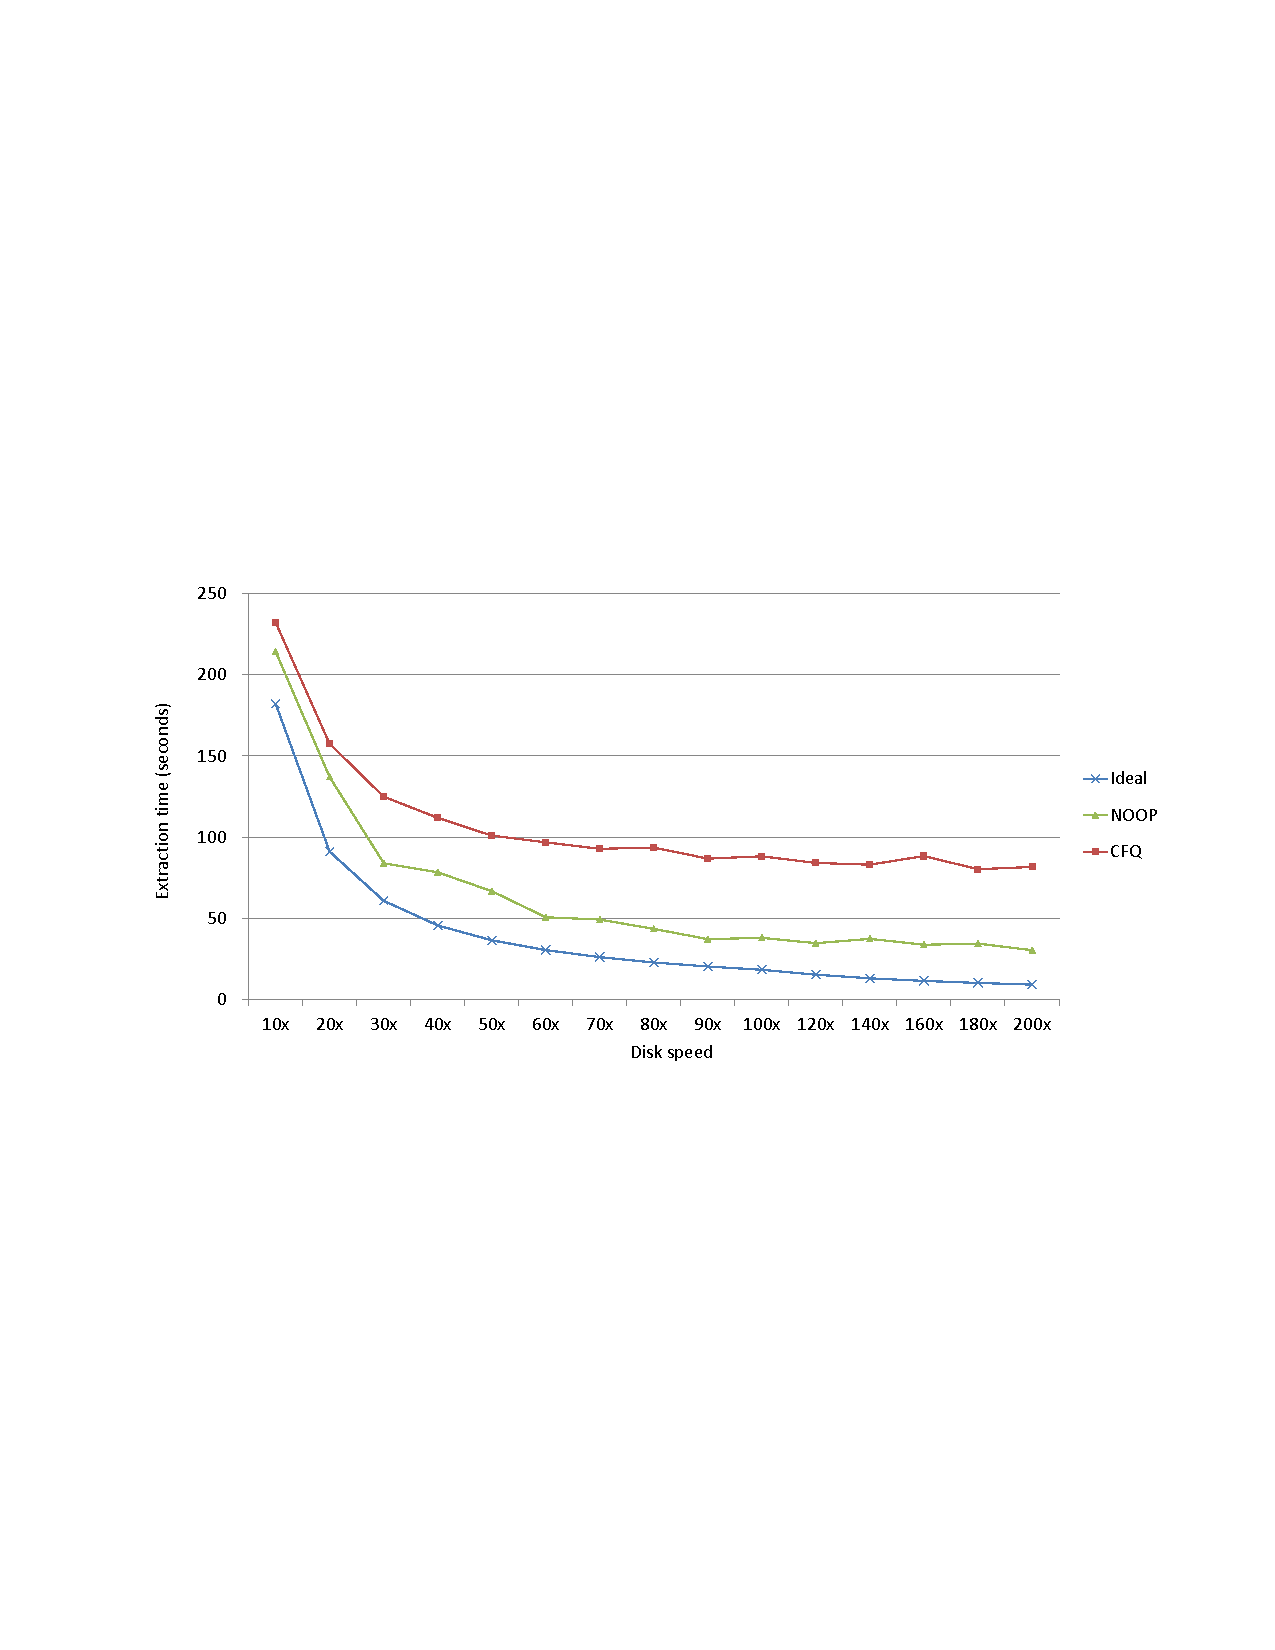
\includegraphics[trim=2cm 10cm 2cm 9.5cm, width=\textwidth]{figures/ch5-predicted-extraction-time.pdf}
	\caption{\label{fig:ch5-predicted-extraction-time}Predicted extraction time.}
\end{figure}

\begin{figure}[htpb]
	\centering
	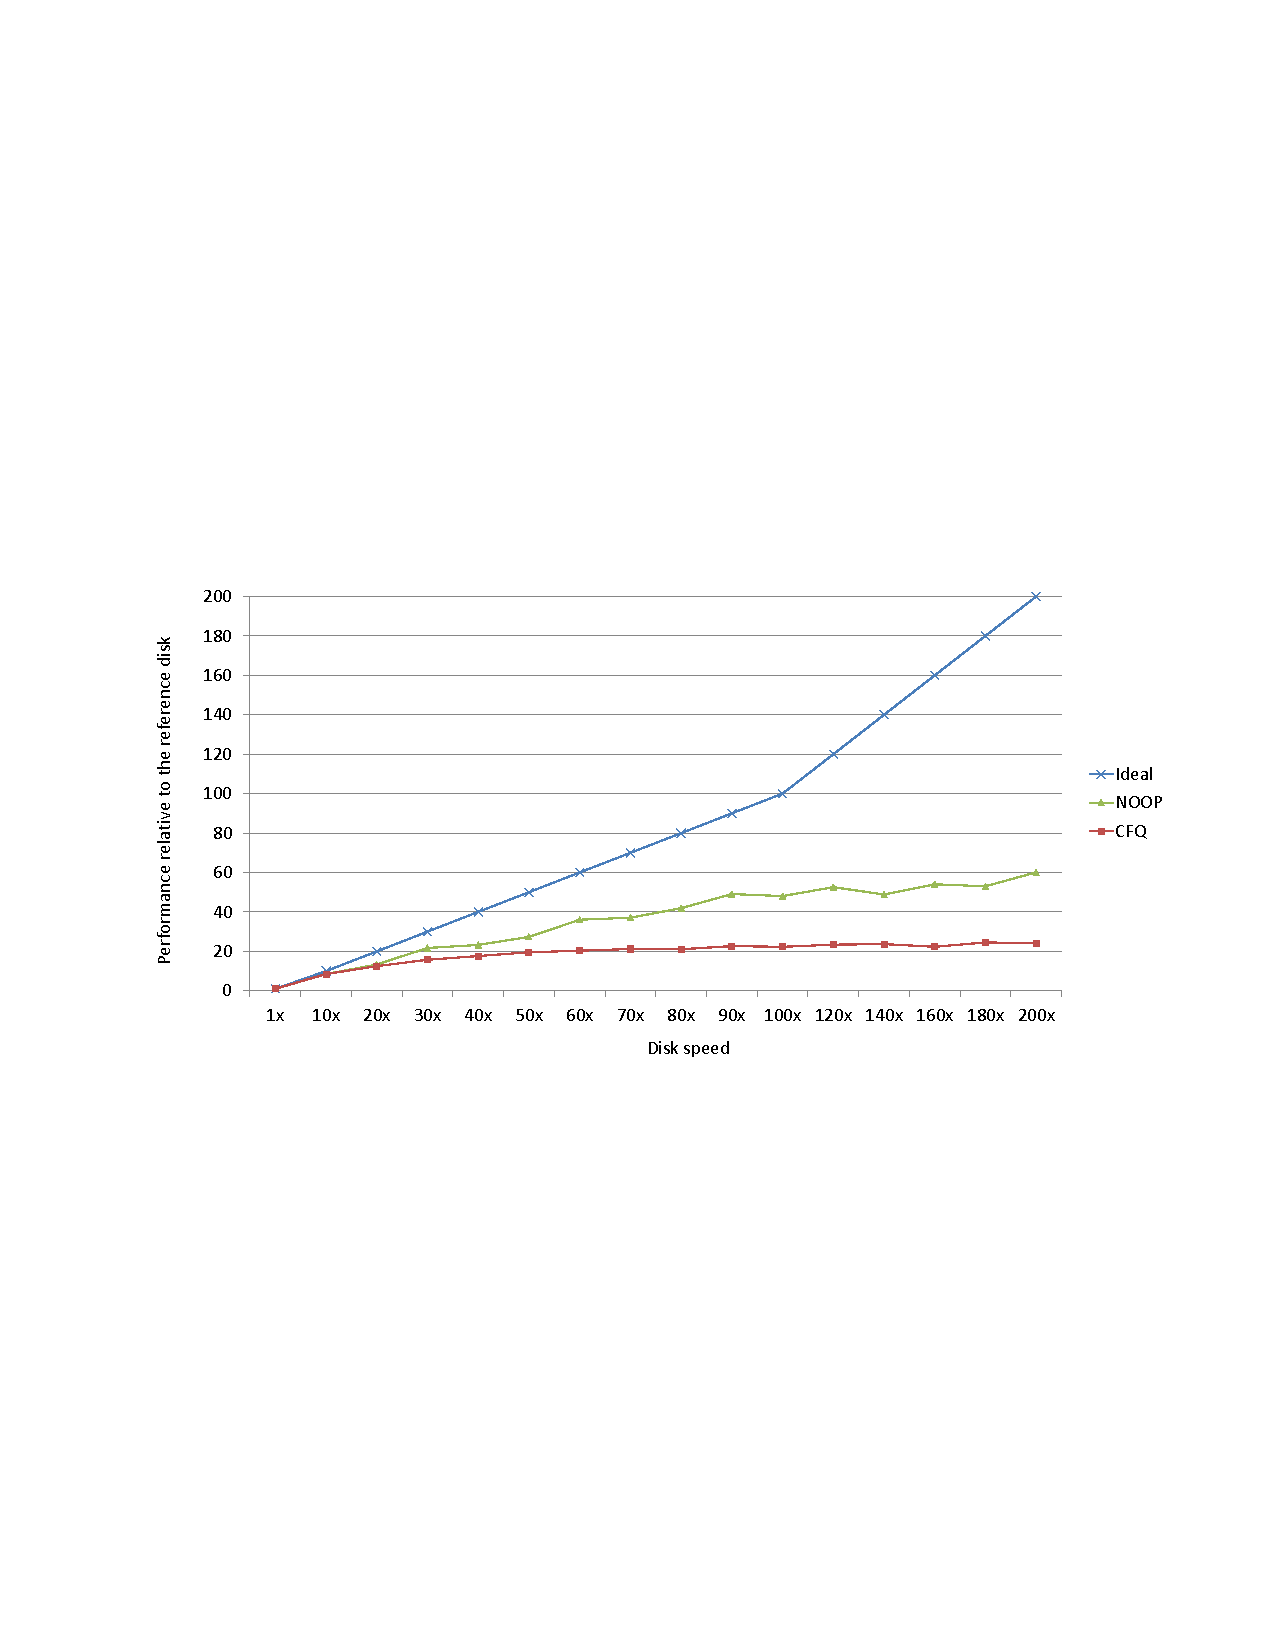
\includegraphics[trim=2cm 10cm 2cm 9.5cm, width=\textwidth]{figures/ch5-speedup-over-reference.pdf}
	\caption{\label{fig:ch5-speedup-over-reference}Speedups over the reference disk.}
\end{figure}


\subsection{Simulating Systems with Different CPU Speeds}
\label{sec:ch5-different-CPU-speeds}

By adjusting the rate at which the virtual system time advances, the proposed full-system co-simulator can trick the Linux OS into thinking that it is running on systems with different CPU speeds than the simulation host. For example, if the system time is advanced by one second for every two seconds that the Linux OS is in the running mode, then to the Linux OS the CPU would appear to be twice as fast as the real CPU that is on the simulation host. During the duration of the one second virtual system time, the CPU will have actually completed the amount of work that it can do in two seconds real-world clock time. With this capability of simulating systems with different CPU speeds, the proposed full-system co-simulator can be used for conducting sensitivity tests regarding what effects the CPU speeds will have to the overall system performance.

The common conception is that video encoding tasks are CPU-bound workloads. In the following use case, the ability of simulating systems with different CPU speeds is used to show that the performance of disk I/O subsystems could become the bottleneck for video encoding tasks. In the following experiments, the virtual storage device being simulated is the IBM 08K0383 36GB hard disk drive. The ext3 file system is used and is mounted with the sync option. The file system is recreated before each test run. The I/O scheduler used is the NOOP scheduler. The workload is generated by running 5 duplicates of the ffmpeg program (version 0.7.6) encoding the 300-frame standard MPEG CIF video test sequence Foreman~\cite{FFmpeg:2013}. The original RAW video is in YCBCR 4:2:0 format and it is encoded to the AVC/H.264 format. The CPU speeds simulated are ranged from 2$\times$ to 10$\times$ in 1$\times$ steps, and from 12$\times$ to 20$\times$ in 2$\times$ steps.

The simulation results are shown in Table~\ref{tab:ch5-encoding-time}. Figure~\ref{fig:ch5-encoding-time} depicts the same results in graphical form. Looking at the trend of the data points from the ``encoding time'' column, we can see that the overall system performance improvements are becoming saturated as the CPU speeds are reaching over seven times. From the disk utilization and CPU utilization data points, observe that the CPU utilization rates drop as the disk is becoming more utilized. In these simulations, the video encoding task has transformed from a CPU-bound workload into an I/O-bound workload as the CPU speed is raised. Such simulated scenarios are not entirely hypothetical since the computation tasks of video processing can be accelerated with the help of application specific acceleration logics~\cite{Wu:2009}, \cite{Wu:2015:ASAP}.


\begin{table}[htbp]%
	\small
	\centering
	\caption{Evaluation results for different CPU speeds}\label{tab:ch5-encoding-time}
	\noindent\begin{tabular}{ccccc}
		\toprule
		\parbox{2cm}{\centering CPU speed} & \parbox{3cm}{\centering Predicted encoding \\ time (seconds)} & \parbox{3cm}{\centering Speedup over \\ CPU with 1$\times$ speed} & \parbox{3cm}{\centering CPU utilization \\ (\% busy)} & \parbox{2.5cm}{\centering Disk utilization \\ (\% busy)} \\
		\midrule
		
		1$\times$ & 78.16 & 1.00 & 99.73 & 28.90 \\
		2$\times$ & 40.10 & 1.95 & 98.22 & 46.98 \\
		3$\times$ & 27.84 & 2.81 & 95.65 & 63.47 \\
		4$\times$ & 22.37 & 3.49 & 92.17 & 76.72 \\
		5$\times$ & 19.85 & 3.94 & 84.23 & 85.72 \\
		6$\times$ & 19.13 & 4.09 & 78.87 & 89.85 \\
		7$\times$ & 18.84 & 4.15 & 72.12 & 92.42 \\
		8$\times$ & 17.50 & 4.47 & 69.99 & 91.78 \\
		9$\times$ & 17.58 & 4.45 & 66.93 & 92.82 \\
		10$\times$ & 17.65 & 4.43 & 65.50 & 93.87 \\
		12$\times$ & 17.13 & 4.56 & 63.36 & 92.95 \\
		14$\times$ & 17.63 & 4.43 & 60.23 & 94.70 \\
		16$\times$ & 17.01 & 4.59 & 58.93 & 95.57 \\
		18$\times$ & 16.80 & 4.65 & 57.21 & 95.57 \\
		20$\times$ & 16.40 & 4.76 & 56.84 & 96.14 \\
		
		\bottomrule
	\end{tabular}
\end{table}%

\begin{figure}[htpb]
	\centering
	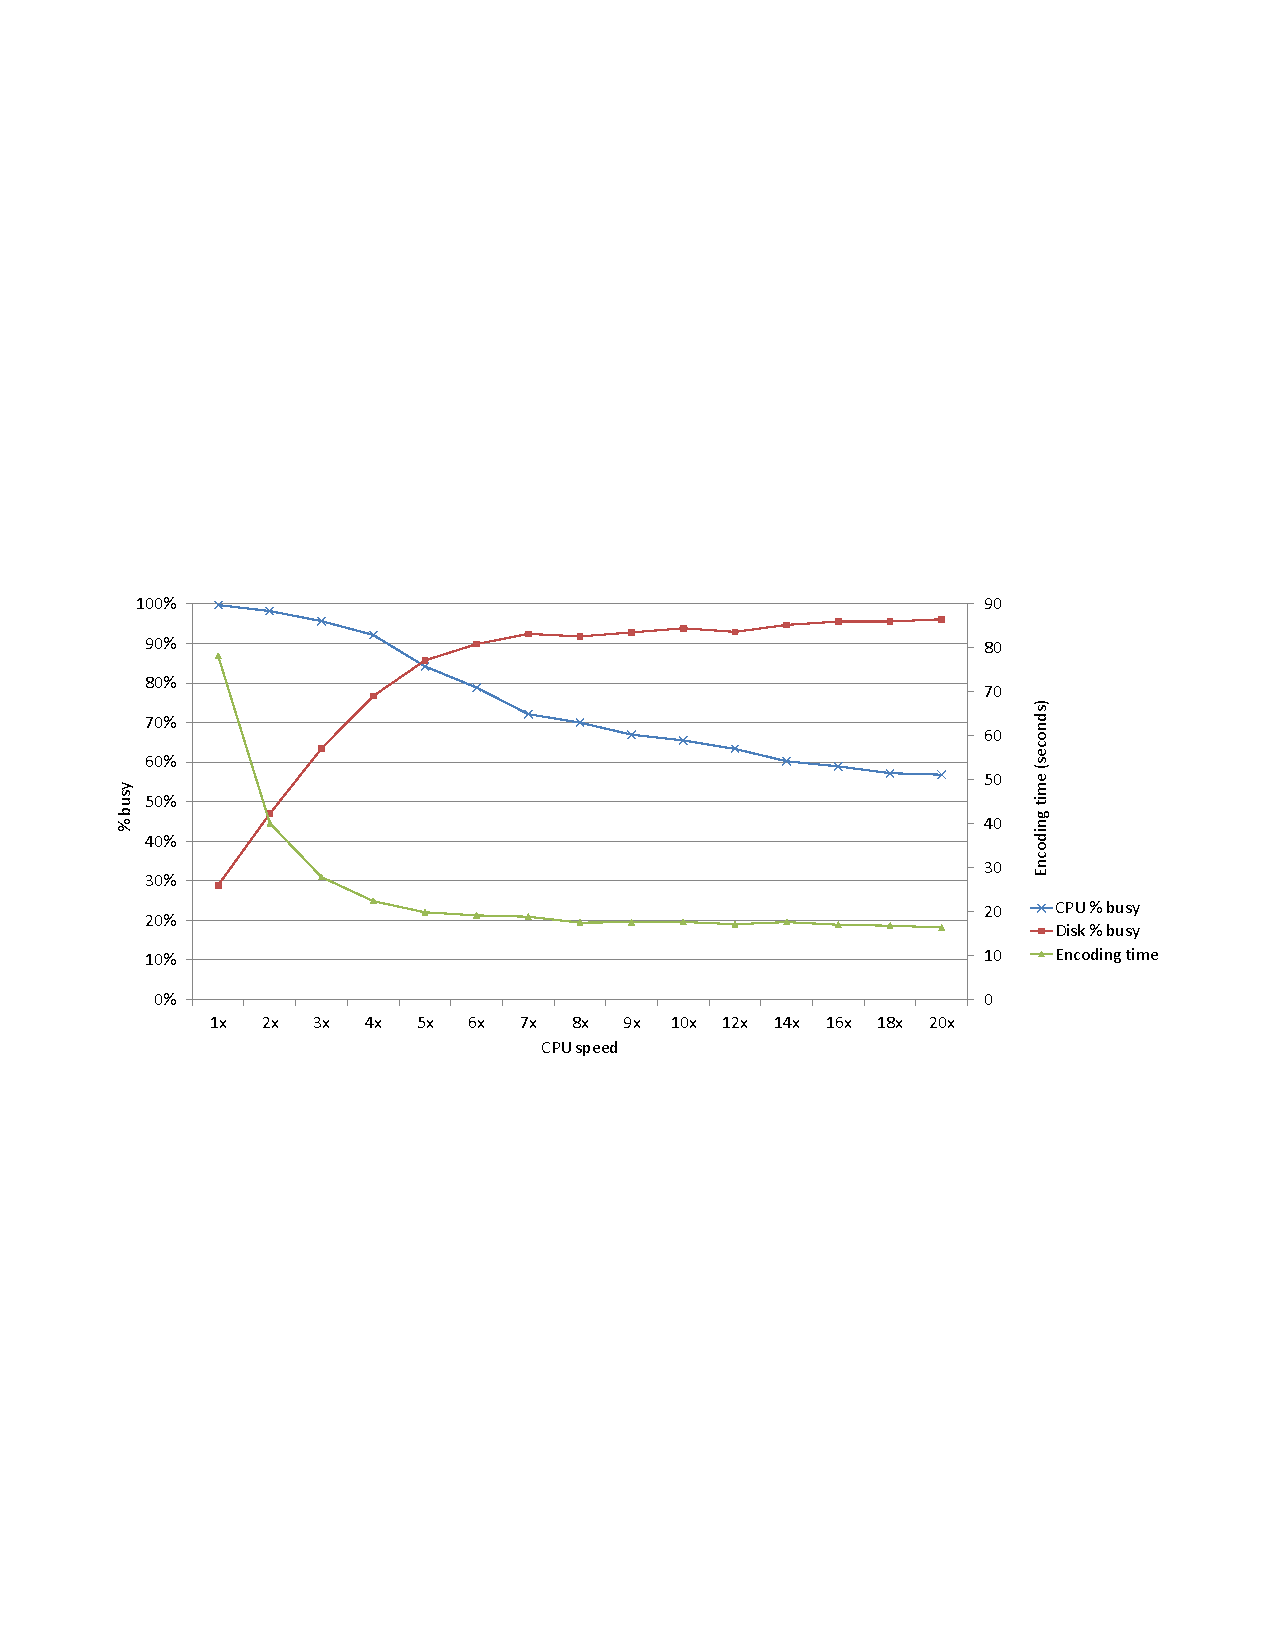
\includegraphics[trim=2cm 10cm 2cm 10cm, width=\textwidth]{figures/ch5-encoding-time.pdf}
	\caption{\label{fig:ch5-encoding-time}Video encoding performance on systems with different CPU speeds.}
\end{figure}
